% Chapter 1

\chapter{A Language of Polynomials} % Main chapter title

\label{Chapter1} % For referencing the chapter elsewhere, use \ref{Chapter1} 

%----------------------------------------------------------------------------------------

% Define some commands to keep the formatting separated from the content 
\newcommand{\keyword}[1]{\textbf{#1}}
\newcommand{\tabhead}[1]{\textbf{#1}}
\newcommand{\code}[1]{\texttt{#1}}
\newcommand{\file}[1]{\texttt{\bfseries#1}}
\newcommand{\option}[1]{\texttt{\itshape#1}}

%----------------------------------------------------------------------------------------

\section{Introduction}

This paper is on the re-framing of the one way function to a matrix multiplication problem - that of multiplying two $3 \times 3$ matrices to form a $6 \times 6$ matrix under a locally concatenative property. The matrix multiplication is a type of law of composition that operates on different layers.

%----------------------------------------------------------------------------------------

\section{Foundations}

There exists a language such that it decides each monomial in the polynomial. In other words, there exists a set of deciders for each monomial in the polynomial where it decides if y is in the monomial. A decider in this term is not of the definition found originally in textbooks but one that is redefined in the below definition.

$\newline$

Given a polynomial

$p(x) = ax^2 + bx + c$

$p(x) = 3x^2 + 4x + 5$

$p(2) = 3(2)^2 + 4(2) + 5$

$p(2) = 12 + 8 + 5$

$\newline$

Let the decider be defined as the following:

$\\ $

Decider is a function $Decider<c \times x^{n}> \equiv c \times x^{n} = y$

such that
$x_1 \times x_2 \times ... \times x_n\ $ where n is equal to degree + constant is tested to be equivalent to y
and $x_1$ is the start
and $x\ degree\ times$ is the finish
then loop around $x_1 to x\ n\ times$ until it stops

For each state, $x_i$, i such that it is between 1 to n, $x_i$ contains a subgroup of size n and for each subgroup, $s_i$, there exists another subgroup and so on and so forth such that there are n layers starting from $x_i$ to 1. This is the same as saying that it is a rational expression.

$\newline$

$\textbf{Examples}$

Decider for $ax^2$ is $Decider<3 (2)^2> \equiv 3(2)^2 = 12$

Decider for $bx$ is $Decider<4 (2)^1> \equiv 4(2)^1 = 8$

Decider for $c$ is $Decider<5 (2)^1> \equiv 5(2)^0 = 5$

$\\ $

\begin{figure}[H]
  \centering
  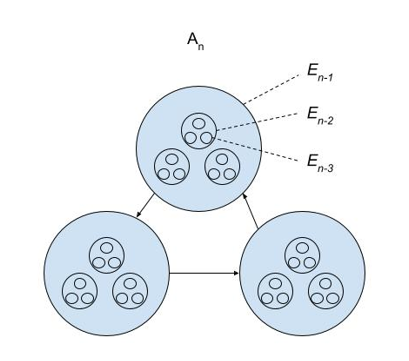
\includegraphics[width=\linewidth]{0101DeciderX3.png}
  \caption{Decider that represents the monomial, $x^3$.}
  \label{fig:0101DeciderX3}
\end{figure}

$\\ $

$\textbf{Theorem}$: A Decider is the equivalent to a cyclic automata

$\\ $

$\textit{Proof}$: Remove the lowest level state, $S_1$ from the bottom then continue removing $S_i$ from i = 2 to n-1 until you get only the states that are at $X_n$.

$\\ $

Remove the top state down from the $S_{n-1}$ for each layer $S_{n-1}$ to $S_(n-n-1)$. This preserves the start and finish state for the layer $x_{n}$. This is a cyclic automaton.

$\\ $

\begin{figure}[H]
  \centering
  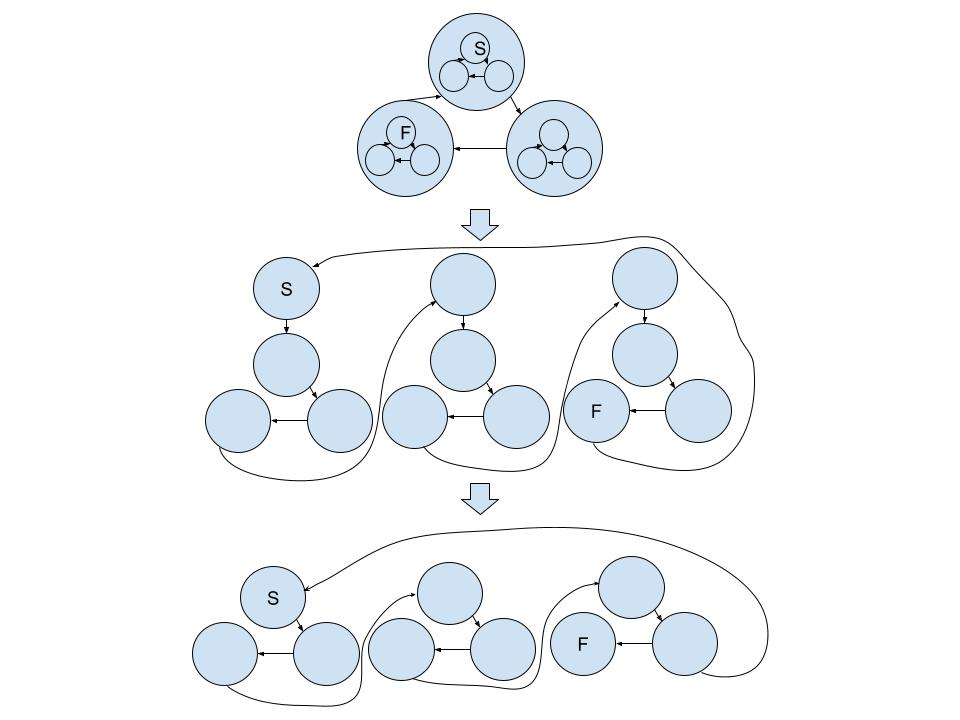
\includegraphics[width=\linewidth]{0102theorem.jpg}
  \caption{Top down removal for equivalence of decider and cyclic automata.}
  \label{fig:0102theorem}
\end{figure}

\section{Monomial of One Variable}

Given the definition of a decider:

Decider is a function $Decider<c x^n> \equiv c x^n = y$

$\\ $

A decider of at least one degree

$Decider< 3 x^4 > \equiv 3x^4 = y$

$\\ $

Contains $Decider<3 x^3> \equiv 3x^3 = y$

Contains $Decider<3 x^2> \equiv 3x^2 = y$

Contains $Decider<3 x^1> \equiv 3x^1 = y$

Contains $Decider<3 x^0> \equiv 3x^0 = y$

Hence it can be generalized to:

$Decider<c x^n>$ contains the sequence set 


$\\ $

There exists a start state and a finish state for each decider.

$\{start,...,finish\}$

$\\ $

$Decider<c x^n>,Decider<c x^{n-1}>,...,Decider<c x^0>$ 
which has a more formal definition called a rational expression. A rational expression on A over K is a semiring described as $\mathcal{E}_{n}$ such that $n\geq0$ where A is an alphabet (in our case a finite set of integers) and K is a commutative semiring. This means the following in terms of the decider

$\\ $

$Decider<c x^n>$ = $\mathcal{E}_{n}$

Contains $Decider<c x^{n-1}>$ = $\mathcal{E}_{n-1}$

...

Contains $Decider<c x^{1}>$ = $\mathcal{E}_{1}$

Contains $Decider<c x^0>$ = $\mathcal{E}_{0}$

$\\ $

The formal definition of a rational expression is defined below.

$\\ $

$\textbf{Definition. }$ $A_n = A_{n-1} \cup  {\left\{  E^* | E \in \mathcal{E}_{n-1}, (E,1)=0 \right\}}$

$\\ $

Here, $A_n$ is the set of monomials in the polynomial. $A_{n-1}$ are the monomials of degree n-1 and less of the polynomial and the set ${\left\{  E^* | E \in \mathcal{E}_{n-1}, (E,1)=0 \right\}}$ is equivalent to $Decider<cx^n>$ or equivalently the top of a single state of a decider.

$\\ $

\begin{figure}[H]
  \centering
  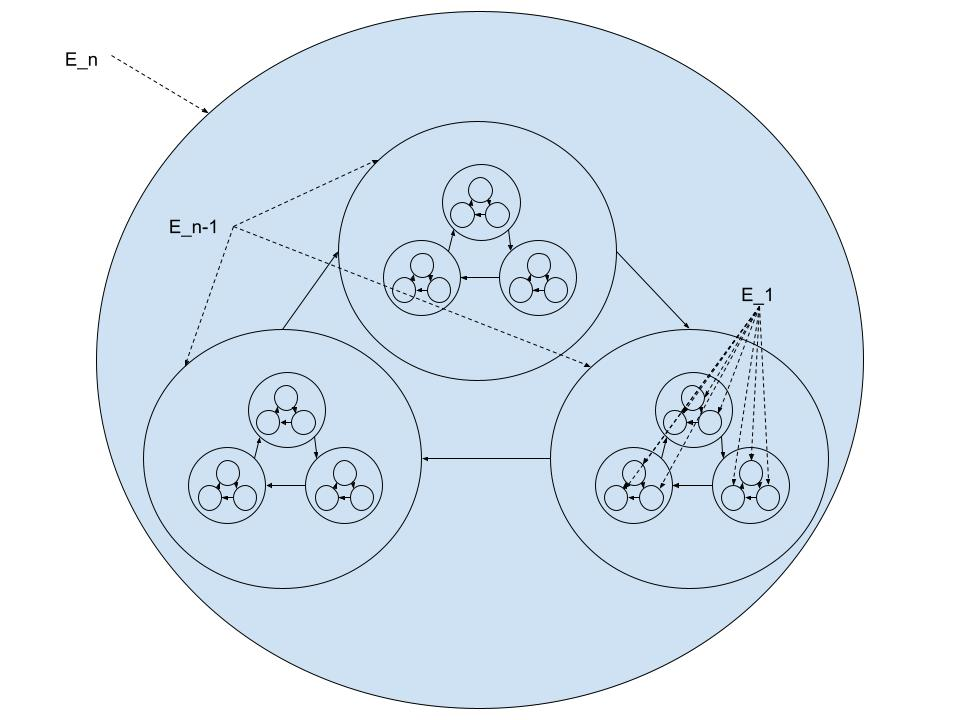
\includegraphics[width=\linewidth]{0103RationalExpression.jpg}
  \caption{Visual example of what $\mathcal{E}_n$ of a rational expression.}
  \label{fig:0103RationalExpression}
\end{figure}
Figure \ref{fig:0103RationalExpression} Visual example of $\mathcal{E}_n$ of a rational expression.

$\\ $

A rational function is defined as the following: 

$\\ $

K[x] and K[[x]]. Let K[[x]] describe a set of deciders as a polynomial representation. S is an element of K[[x]] meaning S is a decider.

$\\ $

S = $\sum_{n\geq 0}{a_n x^n}$

$\\ $


\section{Addition}

\begin{figure}[H]
  \centering
  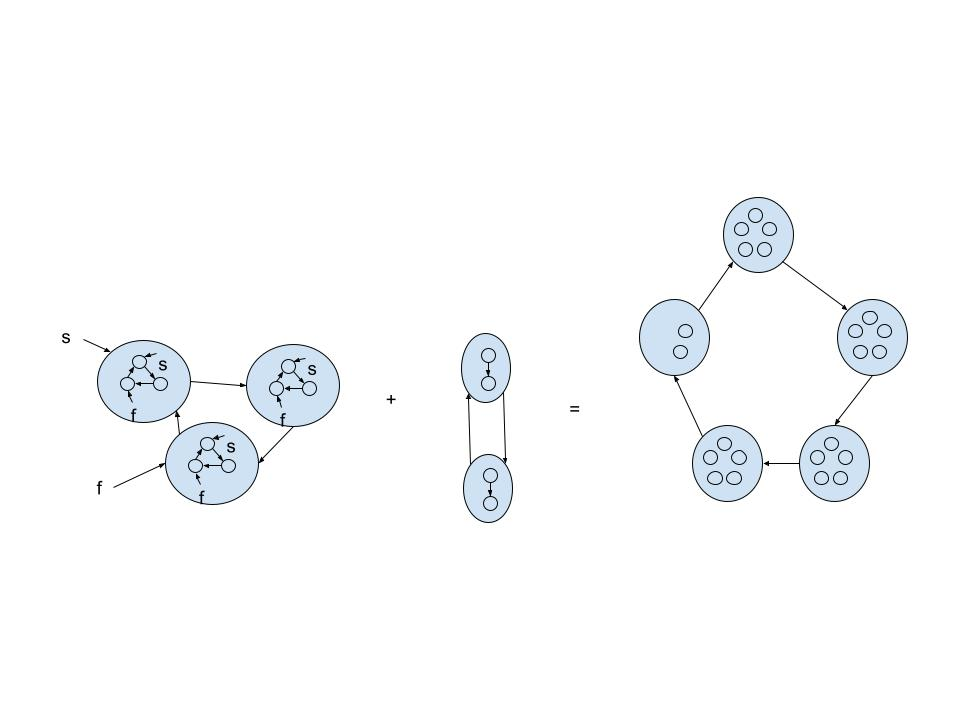
\includegraphics[width=\linewidth]{0104Addition.jpg}
  \caption{Addition of two deciders. The gradient of the circles remain the same after adding the two deciders together as the degree remains the same.}
  \label{fig:0104Addition}
\end{figure}

Given the first example:

$\\ $

$p(x)=3 x^2+4 x+5$

$p(2)=3(2)^2+4(2)+5$

$p(2)=12+8+5$

$\\ $

$m2=Decider<3 x^2>=3x^2$

$m1=Decider<4 x^1>=4 x$

$m0=Decider<5 x^0>=5$

$\\ $

Generalized to $m_x$ where x is the degree

Given polynomial functions, $p_1$ and $p_2$, they are commutative

$p_1(x)=m_a+...+m_0$

$p_2(x)=n_b+...+n_0$

$p_1(x)+p_2(x)=m_a+n_b+(m_{x+1}+n_{y+1})+...+(m_x+n_y)+...+(m_0+n_0)$ where $x=y$

$Decider<c_x x d_x>+Decider<c_y x d_y>$

$=Decider<c_x+c_y,x,d_x>=Deciders<c_x+c_y,x,d_y>$

$\implies d_x=d_y$

\section{Product}

\begin{figure}[H]
  \centering
  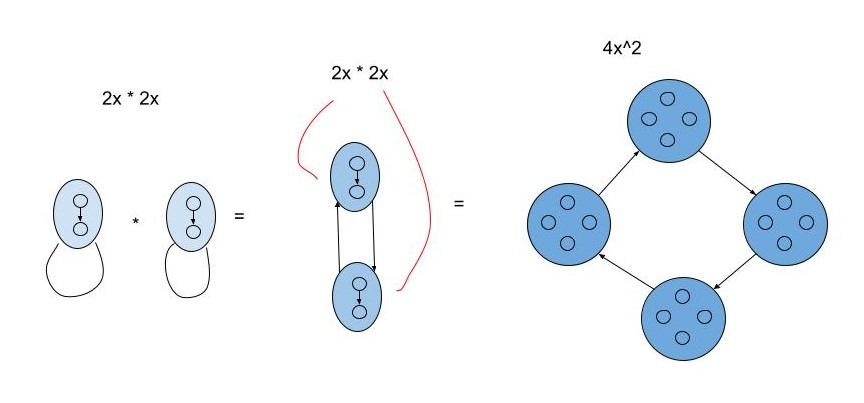
\includegraphics[width=\linewidth]{0105Product.jpg}
  \caption{Product of two deciders. The gradient of the circles get denser after adding the two deciders together as the degree increases.}
  \label{fig:0105Product}
\end{figure}

Given two monomials in the language, a and b, the product of a and b is also in the language.

$\\ $

Given $Decider<c_x x d_x>$ and $Decider<c_y x d_y>$ is in language L

Show that the product $Decider<(c_x+c_y) x d_x\times d_y>$ is in L

$Decider<c_x x d_x> \times Decider<c_y x d_y>$

$=c_x x d_x c_y x d_y$

$=c_x  x d_x+d_y$

$=(c_x+c_y) x (d_x+d_y)$ is in L

$=Decider<(c_x+c_y) x (d_x+d_y)>$

\section{Problem with Matrices}

An important problem arising from deciders is representing them as matrices. The problem can be reformulated as the following: given a polynomial p of x, show that the monomial deciders represented in the language can't be contained in a finite matrix after a set number, n, such that $x^n$.

$\\ $

$\left[ n\times n \right]\left[ n\times n \right]=\left[ m\times m \right]$ such that $m \neq n$ and $m,n\geq 0$ and $m \leq n$

$\\ $

The focus of this article pertains to the question of whether or not there exists structures with certain properties that allow law of compositions to handle the above statement. The reason why this seems feasible is because of the following proposition found in Retenaur(66).

$\\ $

$\textit{Proposition.}$ Given a proper square matrix M over $\mathcal{E}$, there exist matrices $M_1$, $M_2$ of the same size as M over $\mathcal{E}$ such that $M_1 ~1 + MM_1$ and $M_2~1+M_2M$. In particular if K is a ring, 1 - M is an invertible modulo ~.

\section{Multivariable Monomials}

\begin{figure}[H]
  \centering
  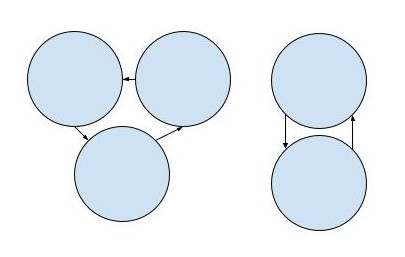
\includegraphics[width=\linewidth]{0106Multivariables.jpg}
  \caption{Multivariable monomial deciders can be seen treated as parallel processes running next to each other.}
  \label{fig:0106Multivariable}
\end{figure}

A monomial with more than one variable can be treated the same way as handling single variables at different degrees.

$\\ $

Addition gives the following:

$\\ $

$Decider<x^6yz^3> + Decider<x^6yz^3> = Decider<2x^6yz^3>$

$\\ $

Multiplication of the decider of the same degree gives the following:

$\\ $

$Decider<cx^n> \times Decider<cy^n> \times Decider<cz^z>$

$\equiv Decider<cx^n * cy^n * cz^n>$

$\equiv Decider<cxyz^{3n}>>$

where c is some constant

$\\ $

Multiplication of the decider of the different degrees gives the following:

$\\ $

$Decider<cx^n> \times Decider<cy^m> \times Decider<cz^l>$

$\equiv Decider<cx^n * cy^m * cz^l>$

$\equiv Decider<cx^{n+m+l}>$

where c is some constant

$\\ $

Given $Decider<3xy^2>$ and $Decider<7x^7y^{-1}>$

$\\ $

$Decider<3xy^2> \times Decider<7x^7y^{-1}> = Decider<21x^8y>$

$\\ $

Representing a multivariable monomial of different degrees is a similar line of thought. There are many representations of them, however, this article will choose the simplest and have them separate as seen in figure 1.6. In this manner, multivariable monomials are a set of individual one variable monomials running simultaneously.

\section{Generalized Monomial Deciders}

\begin{figure}[H]
  \centering
  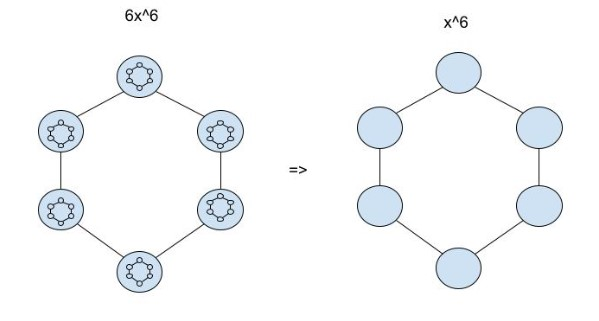
\includegraphics[width=\linewidth]{0107Generalized.jpg}
  \caption{Generalization of a monomial decider.}
  \label{fig:0107Generalized}
\end{figure}

A decider can be represented as the top layer only if short hand notation is necessary.

$\\ $

Given a Decider<m(x)> where m(x) is a monomial, keep the top layer $S_n$ in $\mathcal{E_n}$. This is called the generalized monomial decider.

\section{Concentric Monomial Deciders}

\begin{figure}[H]
  \centering
  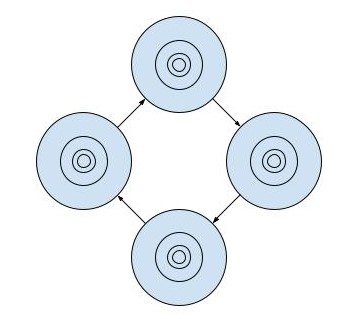
\includegraphics[width=\linewidth]{0108Concentric.jpg}
  \caption{A concentric monomial decider is a generalized monomial decider with details missing.}
  \label{fig:0108Concentric}
\end{figure}

Generalization results in an interesting property if monomial decider is required to get in more depth. The top layer that remains from generalization remains the same and still forms a cycle, however, each state has one state and so forth up to n-1 depth.
 
\section{Constants}

\begin{figure}[H]
  \centering
  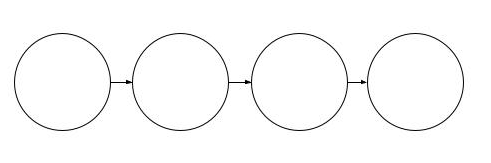
\includegraphics[width=\linewidth]{0109Constants.png}
  \caption{A constant represented as monomial decider, $Decider<c x^0>$.}
  \label{fig:0109Constants}
\end{figure}

Given a constant, c, of a polynomial: f(x) = c, Constants are seen as linear directed acyclic graphs.

$\\ $

$Decider<c x^0> \equiv c = y$

$\\ $

Addition gives the following:

$Decider<c_1 x^0> + Decider<c_2 x^0> \equiv Decider<(c_1+c_2) x^0> \equiv Decider<c_1 + c_2>$

$\\ $

Multiplication gives the following: 

$Decider<c_1 x^0> \times Decider<c_2 x^0> \equiv Decider<c_1 c_2 x^0> \equiv Decider<c_1 c_2>$

$\\ $

There is no state in the decider where it loops back to the start. 

\section{Division}

Division of monomial deciders

$\\ $

\begin{figure}[H]
  \centering
  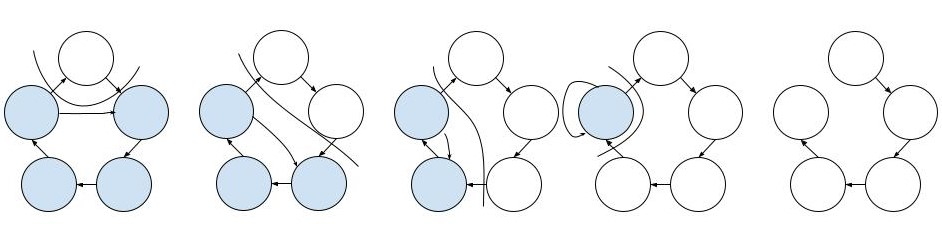
\includegraphics[width=\linewidth]{0110x5.jpg}
  \caption{$Decider<x^5/x>$ to $Decider<x^5/x^5>$.}
  \label{fig:0110x5overx}
\end{figure}

$Decider<x^5 / x> \equiv Decider<x^5>/Decider<x^1>$

$\\ $

$Decider<x^5 / x^2> \equiv Decider<x^5>/Decider<x^2>$

$\\ $

$Decider<x^5 / x^3> \equiv Decider<x^5>/Decider<x^3>$

$\\ $

$Decider<x^5 / x^4> \equiv Decider<x^5>/Decider<x^4>$

$\\ $

$Decider<x^5 / x^5> \equiv Decider<x^5>/Decider<x^5>$

$\\ $

In the following examples, $x_i \neq x_j$, meaning $x_i$ is of a different representation than $x_j$

$\\ $

$Decider<x^5/x^1> \equiv$
 {sequence of permutations of $x_i,x_j$ such that the count of i is 4 and j is 1}

$\\ $
 
$Decider(<x^5/x^2> \equiv$
 {sequence of permutations of $x_i,x_j$ such that the count of i is 3 and j is 2}
 
$\\ $

$Decider<x^5/x^3> \equiv$
 {sequence of permutations of $x_i,x_j$ such that the count of i is 2 and j is 3}

$\\ $
 
$Decider<x^5/x^4> \equiv$ 
 {sequence of permutations of $x_i,x_j$ such that the count of i is 1 and j is 4}

$\\ $
 
$Decider<x^5/x^5> \equiv$
 {sequence of permutations of $x_i,x_j$ such that the count of i is 0 and j is 5} 

$\\ $

\section{Multiple Divisions}

\begin{figure}[H]
  \centering
  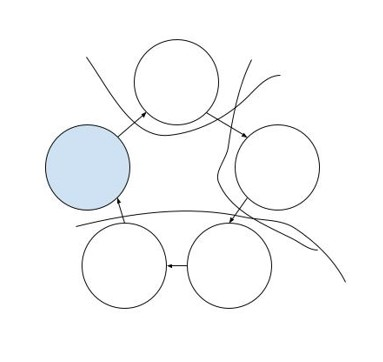
\includegraphics[width=\linewidth]{0111MultipleDivisions.jpg}
  \caption{$Decider<x^5/x/x/x^2>$}
  \label{fig:0111MultipleDivisions}
\end{figure}

$\\ $

Given multiple operations of division, this forms a topological space where the order of operations are ignored.

$\\ $

$x^5/x^2/x/x=x^5/x^2/x^2$.

$Decider<x^5/x^2/x^1/x^1> \equiv Decider<x^5/x^2/x^2>$
 
\section{Equivalence}

\begin{figure}[H]
  \centering
  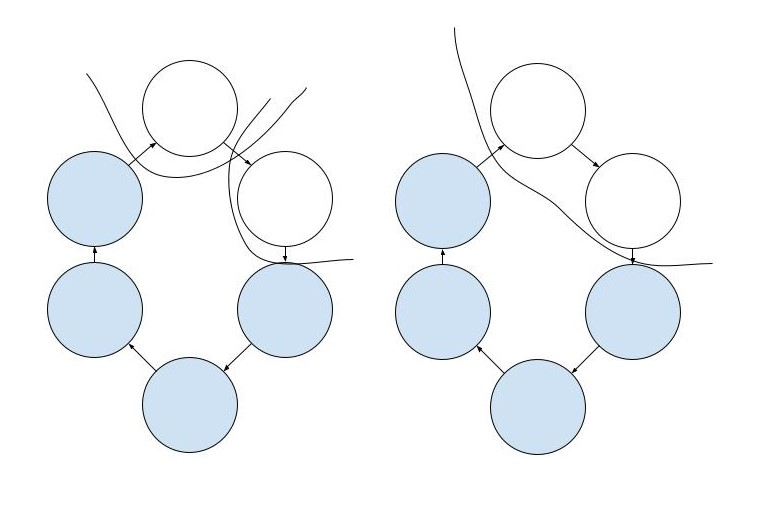
\includegraphics[width=\linewidth]{0112Equivalence.jpg}
  \caption{$Decider<x^6/x^2>$}
  \label{fig:0112Equivalence}
\end{figure}

$Decider<x^6/x^1/x^1> ~ Decider<x^6/x^2>$

$\\ $
Determining if y is in f x is easy if we are given any monomial decider in the set of the language of polynomials and their representations has the possibility to give different representations if we consider them as representations of the function f of x.

$\\ $

$Decider<x^6/x^1/x^1> \sim Decider<x^6/x^2>$ in that they decide if y is in m(x) = $x^6/Q$

$\\ $

$\textbf{Theorem of Equivalence}$. Something on lines of $Decider<x^6/x^1/x^1> = Decider<x^6/x^2>$ such that there is some x such that the monomial represented by both deciders exists where f of x = y.

\section{Reversing}

$\\ $

$Decider<x^6/x^1/x^1> \equiv $sequence of permutations such that it is equal to $\sum_{i}^{n-1}{i}$

$\\ $

$Decider<x^6/x^2> \equiv $ sequence of permutations of $x_i$, $x_j$ such that it equals n-1.

$\\ $

Is shown that by the permutation of the order of operations that $Decider<x^6/x^1/x^1>$ does not have the same number of permutations as $Decider<x^6/x^2>$

$\\ $

$\textbf{Theorem of Reversing}$. Given two representations, a,b in $Decider<m(x)/Q>$ where m(x) is monomial and Q is the division operations such that m(x)/Q $\geq $ 1, a != b implies that they don't have the same quotients space.

$\\ $

$\textit{Proof}.$ Proof by construction visually to show a != b.

\begin{figure}[H]
  \centering
  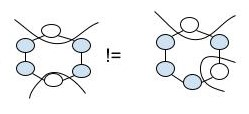
\includegraphics[width=\linewidth]{0113Reversing.jpg}
  \caption{Two possible representations of $Decider<x^6/x/x>$.}
  \label{fig:0113Reversing}
\end{figure}

The two representations in 1.13 don't have the same quotient space and hence a != b.

\section{Corollary of Reversing}

Given a starting point of decider, the path the decider takes to decide if y is in the monomial, m(x) is unique to each representation. 

$\\ $
$\textbf{Corollary}$. Given a decider, d, in $Decider<m(x)>$ then there is path, p, that exists for d such that p = Path(d) = $s_1,s_2,...,s_i,...,s_n$ where i is count of the states in the decider of m(x).

$\\ $

$\textit{Example}$. Choose some x such that it is in path of $Decider<x^6/x^2>$ where $p = 001111$ then the following graph is what the decider is represented as.

\begin{figure}[H]
  \centering
  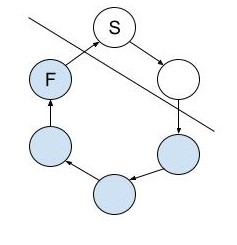
\includegraphics[width=\linewidth]{0114CorollaryOfReversing.jpg}
  \caption{Path of one representation of $Decider<x^6/x^2>$.}
  \label{fig:0114CorollaryOfReversing}
\end{figure}

\section{Godel's Theorem}

We see that there exists two statements from these theorems

$\\ $

1. $x = x$ from a theorem of equivalence

2. $x != x$ from a theorem of reversal

$\\ $

$\textbf{Example}$: Given some $d_1$,$d_2$,$d_3$,...,infinity in decision functions in $Decider<m(x)>$

$\\ $

1. $d_1 = d_2 = d_3 = ... = infinity$

2. $d_1 != d_2 != d_3 = ... != infinity$

$\\ $

The different representations of a monomial through the language of monomial deciders will give the problem of undecidability. This means that despite many formal definitions of the monomial decider, there is no way to solve the problem of finding a specific representation of a monomial decider without having to guess or apply some sort of probability to it. Relating to the real line, given a real line a,b a $\leq$ b, there is infinite choices between a and b. As long as b and a $\geq $ 0, there requires some sort of probability of choosing some specific number that is between a and b.

\section{Reframing The One Way Function}

A probability exists to find a certain monomial decider in the set of it's variations. A/B = Probability where A is the monomial decider we want and B is the number of all the variations.

$\\ $

Example:
d1,d2,...,d6 in deciders 1,x,6 ,D, such that di are all distinct
Choose one of the deciders in D through probability
Probability of choosing d in D is 1/6 so 0.16666667
We'll call this picking a function and every time we call this function, the probability is mulltiplied such that it is n k. As an example, if we call the picking function twice using the example above, we have 1/6 1/6 = 1/36 = 6 2.

$\\ $

This is formally known as the one way function.

\section{Theorem of Infiniteness}

Given that, if we can show for any language it abides a theorem of equivalence and a theorem of reversal and they both have infinite representations, we know that we need some sort of probability to choose a specific representation of a monomial decider. We'll call this a theorem of infiniteness because if we can show that some language is infinite, it will require some sort of guess to pick something unique out of all the things it represents, generates, or describes. In other words, you can't map infinity to infinity directly for you must map infinity to something discrete and something discrete to infinity.

Theorem
A mapping must be from infinity to discrete representation to discrete representation to infinity.

Given any representation of infinity,
Suppose a mapping infinity to infinity exists.
Then this map is equivalent to infinity because 
infinity contains this map.
Here, infinity is represented as $\ast. \ast contains \ast -> \ast.$

Intuition

Given Decider c,x,d and d is infinity,
Decider c,x,d contains Decider c,x,d 1
d 1 is then infinity too.


\subsection{References}

The \code{biblatex} package is used to format the bibliography and inserts references such as this one \parencite{Reference1}. The options used in the \file{main.tex} file mean that the in-text citations of references are formatted with the author(s) listed with the date of the publication. Multiple references are separated by semicolons (e.g. \parencite{Reference2, Reference1}) and references with more than three authors only show the first author with \emph{et al.} indicating there are more authors (e.g. \parencite{Reference3}). This is done automatically for you. To see how you use references, have a look at the \file{Chapter1.tex} source file. Many reference managers allow you to simply drag the reference into the document as you type.

Scientific references should come \emph{before} the punctuation mark if there is one (such as a comma or period). The same goes for footnotes\footnote{Such as this footnote, here down at the bottom of the page.}. You can change this but the most important thing is to keep the convention consistent throughout the thesis. Footnotes themselves should be full, descriptive sentences (beginning with a capital letter and ending with a full stop). The APA6 states: \enquote{Footnote numbers should be superscripted, [...], following any punctuation mark except a dash.} The Chicago manual of style states: \enquote{A note number should be placed at the end of a sentence or clause. The number follows any punctuation mark except the dash, which it precedes. It follows a closing parenthesis.}

The bibliography is typeset with references listed in alphabetical order by the first author's last name. This is similar to the APA referencing style. To see how \LaTeX{} typesets the bibliography, have a look at the very end of this document (or just click on the reference number links in in-text citations).

\subsubsection{A Note on bibtex}

The bibtex backend used in the template by default does not correctly handle unicode character encoding (i.e. "international" characters). You may see a warning about this in the compilation log and, if your references contain unicode characters, they may not show up correctly or at all. The solution to this is to use the biber backend instead of the outdated bibtex backend. This is done by finding this in \file{main.tex}: \option{backend=bibtex} and changing it to \option{backend=biber}. You will then need to delete all auxiliary BibTeX files and navigate to the template directory in your terminal (command prompt). Once there, simply type \code{biber main} and biber will compile your bibliography. You can then compile \file{main.tex} as normal and your bibliography will be updated. An alternative is to set up your LaTeX editor to compile with biber instead of bibtex, see \href{http://tex.stackexchange.com/questions/154751/biblatex-with-biber-configuring-my-editor-to-avoid-undefined-citations/}{here} for how to do this for various editors.
